\chapter{Making Of A Cyborg}
\epigraph{What is real? How do you define 'real'? If you're talking about what
you can feel, what you can smell, what you can taste and see, then 'real' is
simply electrical signals interpreted by your brain.}
{Morpheus to Neo - The Matrix}
The mission statement of the NTNU cyborg is ``... to enable communication
between living nerve tissue and a robot. The social and interactive Cyborg
serves as a platform for studying neural signaling properties, robotics and
hybrid bio-robotic machines.'' \cite{ntnu_cyborg}
The work in this thesis is strictly focused on enabling communication, leaving
the robotic and social aspects for later work.
This section presents the design and implementation of a system capable of
communicating with neural tissue and controlling a robot in three parts,
wetware, hardware and most importantly software.
\subsubsection{Concept}
In figure \ref{figOverviewSimple} the conceptual cyborg is shown.
This conceptual cyborg is comprised of three main components: An \emph{MEA}, short
for \emph{Micro Electrode Array} in which a biological neural network is grown.
A \emph{neural interface}, allowing two-way communication between the neural network and
the outside world.
A robotic body, responding to movement commands and equipped with a sensor
allowing it to perceive its environment.
In this concept neural readouts are transformed into a Left and Right signal by
a feed forward neural network, controlling the direction of the robot.
Simultaneously, data retrieved from the sensors of the robot are processed in a
feedback processor and fed back to the neural network.
The conceptual cyborg is a closed loop system: The only input to the system is
what the sensors perceive, which the cyborg in turn acts upon.
\begin{figure}[h]
  \centering
  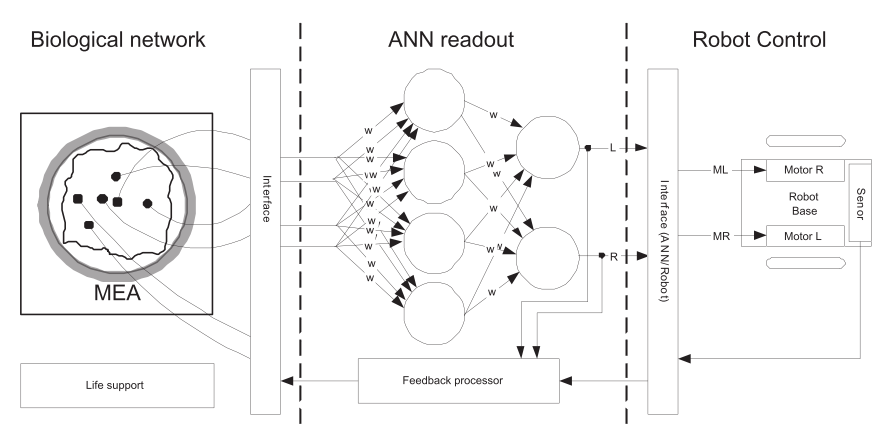
\includegraphics[width=0.7\textwidth]{fig/cyborg_overview.png}
  \caption[Conceptual cyborg]{
    A conceptual model for a cyborg.
    In the conceptual model, a robot equipped with a sensor relays the input
    captured by the sensor to the neurons in form of stimuli generated by the
    feedback processor.
    The resulting dynamics of the neural tissue is then recorded and transformed
    into input values for a feed forward neural network which tells the robot
    which way to move. 
  }
  \label{figOverviewSimple}
\end{figure}
\subsubsection{Architecture}
As shown in figure \ref{figOverview}, the actual cyborg adds a lot of parts
compared to the initial concept.
This design expands on the initial concept of figure \ref{figOverviewSimple}, fleshing
out the ``interface'' box from the conceptual cyborg, juxtaposed in figure
\ref{figJuxta}.
As the conceptual cyborg indicates, what goes on in the box labeled interface is
mostly implementation detail, thus the robot control and reservoir readout is
known as the \emph{core reservoir computer}, differentiating it from the interface
components.
The more detailed overview in figure \ref{figOverview} focuses on the main data loop, depicted as
red and green lines, with red denoting the data pipeline from the reservoir to
the core reservoir loop, and green from core reservoir loop to reservoir.
The expanded architecture reveals a very important detail in the final design:
The closed data loop between neurons and robot extends over network. 
This design choice allows the neural cultures to be safely stored in a
laboratory, which has ramications both in a practical and philosophical sense.
By decoupling the reservoir and reservior computer, the neurons are not
restricted to a single robot.
In fact, the robot does not have to be a physical robot, it can be fully virtual
without the neurons noticing any difference.
Additionally, the reservoir computer can interface with any reservoir as long as
the constraints set by the interfaces are satisfied.
This allows other reservoirs to be used in place of the neurons, both for
testing purposes, and to compare the capabilities of different reservoirs.
\begin{figure}[h!]
  \centering
  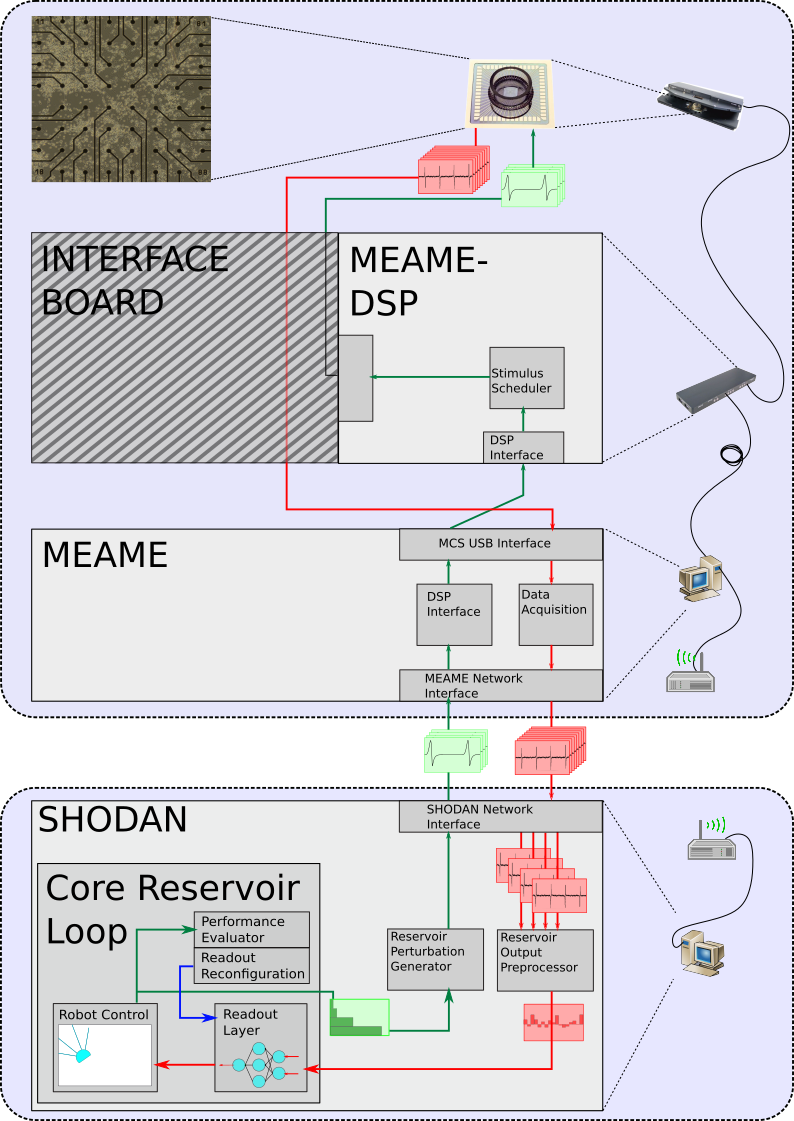
\includegraphics[width=0.7\textwidth]{fig/system3.png}
  \caption[Block diagram overview of the cyborg]{
    The full overview of the cyborg, divided into the three systems: MEAME,
    MEAME-DSP and SHODAN.
    The arrows denote dataflows, where the red arrows show data going from the
    neural tissue to the core reservoir computers, and the green arrows going
    from robot sensors back to the reservoir.
    On the left side the various devices where each system resides on is shown,
    including how they communicate with each other.
    Physical proximity is indicated by the blue tinted box, and as hinted by the
    routers communication crossing this physical gap happens over network.
    (If the colors are hard to see, the red line goes from the MEA to the
    readout layer as indicated by the arrowtips.)
  }
  \label{figOverview}
\end{figure}
%
\clearpage
\begin{figure}[h]
  \centering
  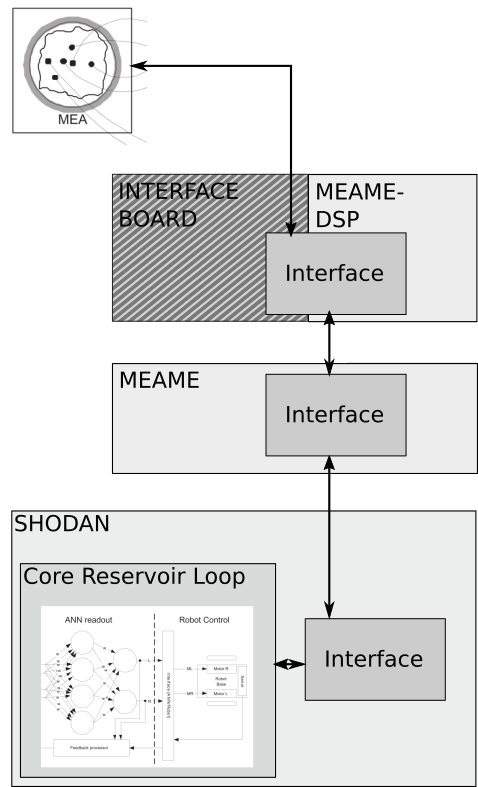
\includegraphics[width=0.5\textwidth]{fig/ConceptMap.png}
  \caption[Conceptual cyborg model compared with implemented]{
    When juxtaposing the pieces of the conceptual cyborg in figure
    \ref{figOverviewSimple} onto the fleshed out design it becomes apparent that the
    interface box makes up a majority of the cyborg.
  }
  \label{figJuxta}
\end{figure}
\section{Wetware}
As opposed to hardware and software, the term wetware describes system
components of biological origin, i.e ``wet'' components.
The wetware of the cyborg is thus the neural networks which are being grown in
MEAs at the department of neuroscience located at the St.Olavs research hospital.
The MEAs are \emph{seeded} by introducing a solution containing neurons that
have formed from stem cells of human origin\cite{TMAC}.
Just after seeding there is no network at all, only a ``soup'' of dissociated
neurons which over the course of several weeks start forming networks.
The activity from these so-called pacemaker neurons can be seen in figure
\ref{pacemaker}.
In the pacemaker figure, each cell in the grid corresponds to one of the
electrodes seen as black lines in figure \ref{frank}
At this stage the monotonic spiking activity tends to be transient, starting and
stopping randomly.
\begin{figure}[h]
  \centering
  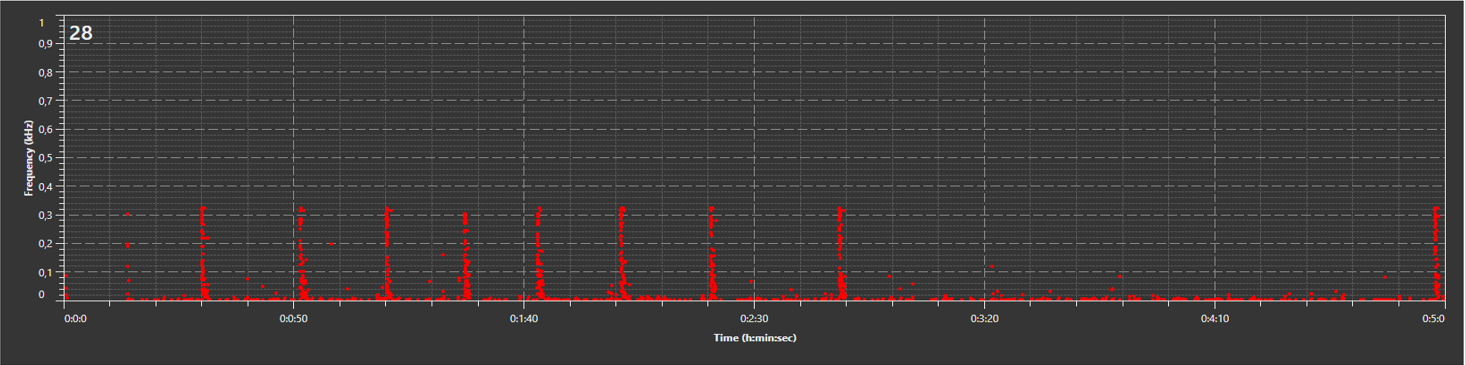
\includegraphics[width=1\textwidth]{fig/tonic.png}
  \caption[Pacemaker bursts]{
    A readout showing spikes from a neural network on an MEA measured on a
    single electrode.
    The spikes follows a ``pacemaker'' pattern for a while, before petering off,
    This pattern typically forms after a few weeks.
    Figure source: \cite{TMAC}
  }
  \label{pacemaker}
\end{figure}
\subsection{Neural Interface}
The \emph{Neural Interface} is the bridge between the biological and digital,
responsible for providing a convenient API (application programming interface)
for reading out digital waveform data and inducing stimuli.
The MEA2100 is built to conduct in-vitro experiments on electrically active cell
cultures such as neurons contained in micro electrode arrays, by measuring and
and inducing voltages with its high precision electrodes.
Although not originally intended for use in close loop systems, the \textit{MEA2100}
system features the necessary hardware to implement a neural interface with the
necessary functionality for a closed loop system.
In addition to voltage and current, the MEA2100 system comes with a life support
module, allowing neural cultures to survive for prolonged experiments for up to
30 minutes.
Figure \ref{labEquip} shows a physical
overview of the components that make up the neural interface, which is also
marked in figure \ref{figOverview}.
\begin{figure}[h!]
  \centering
  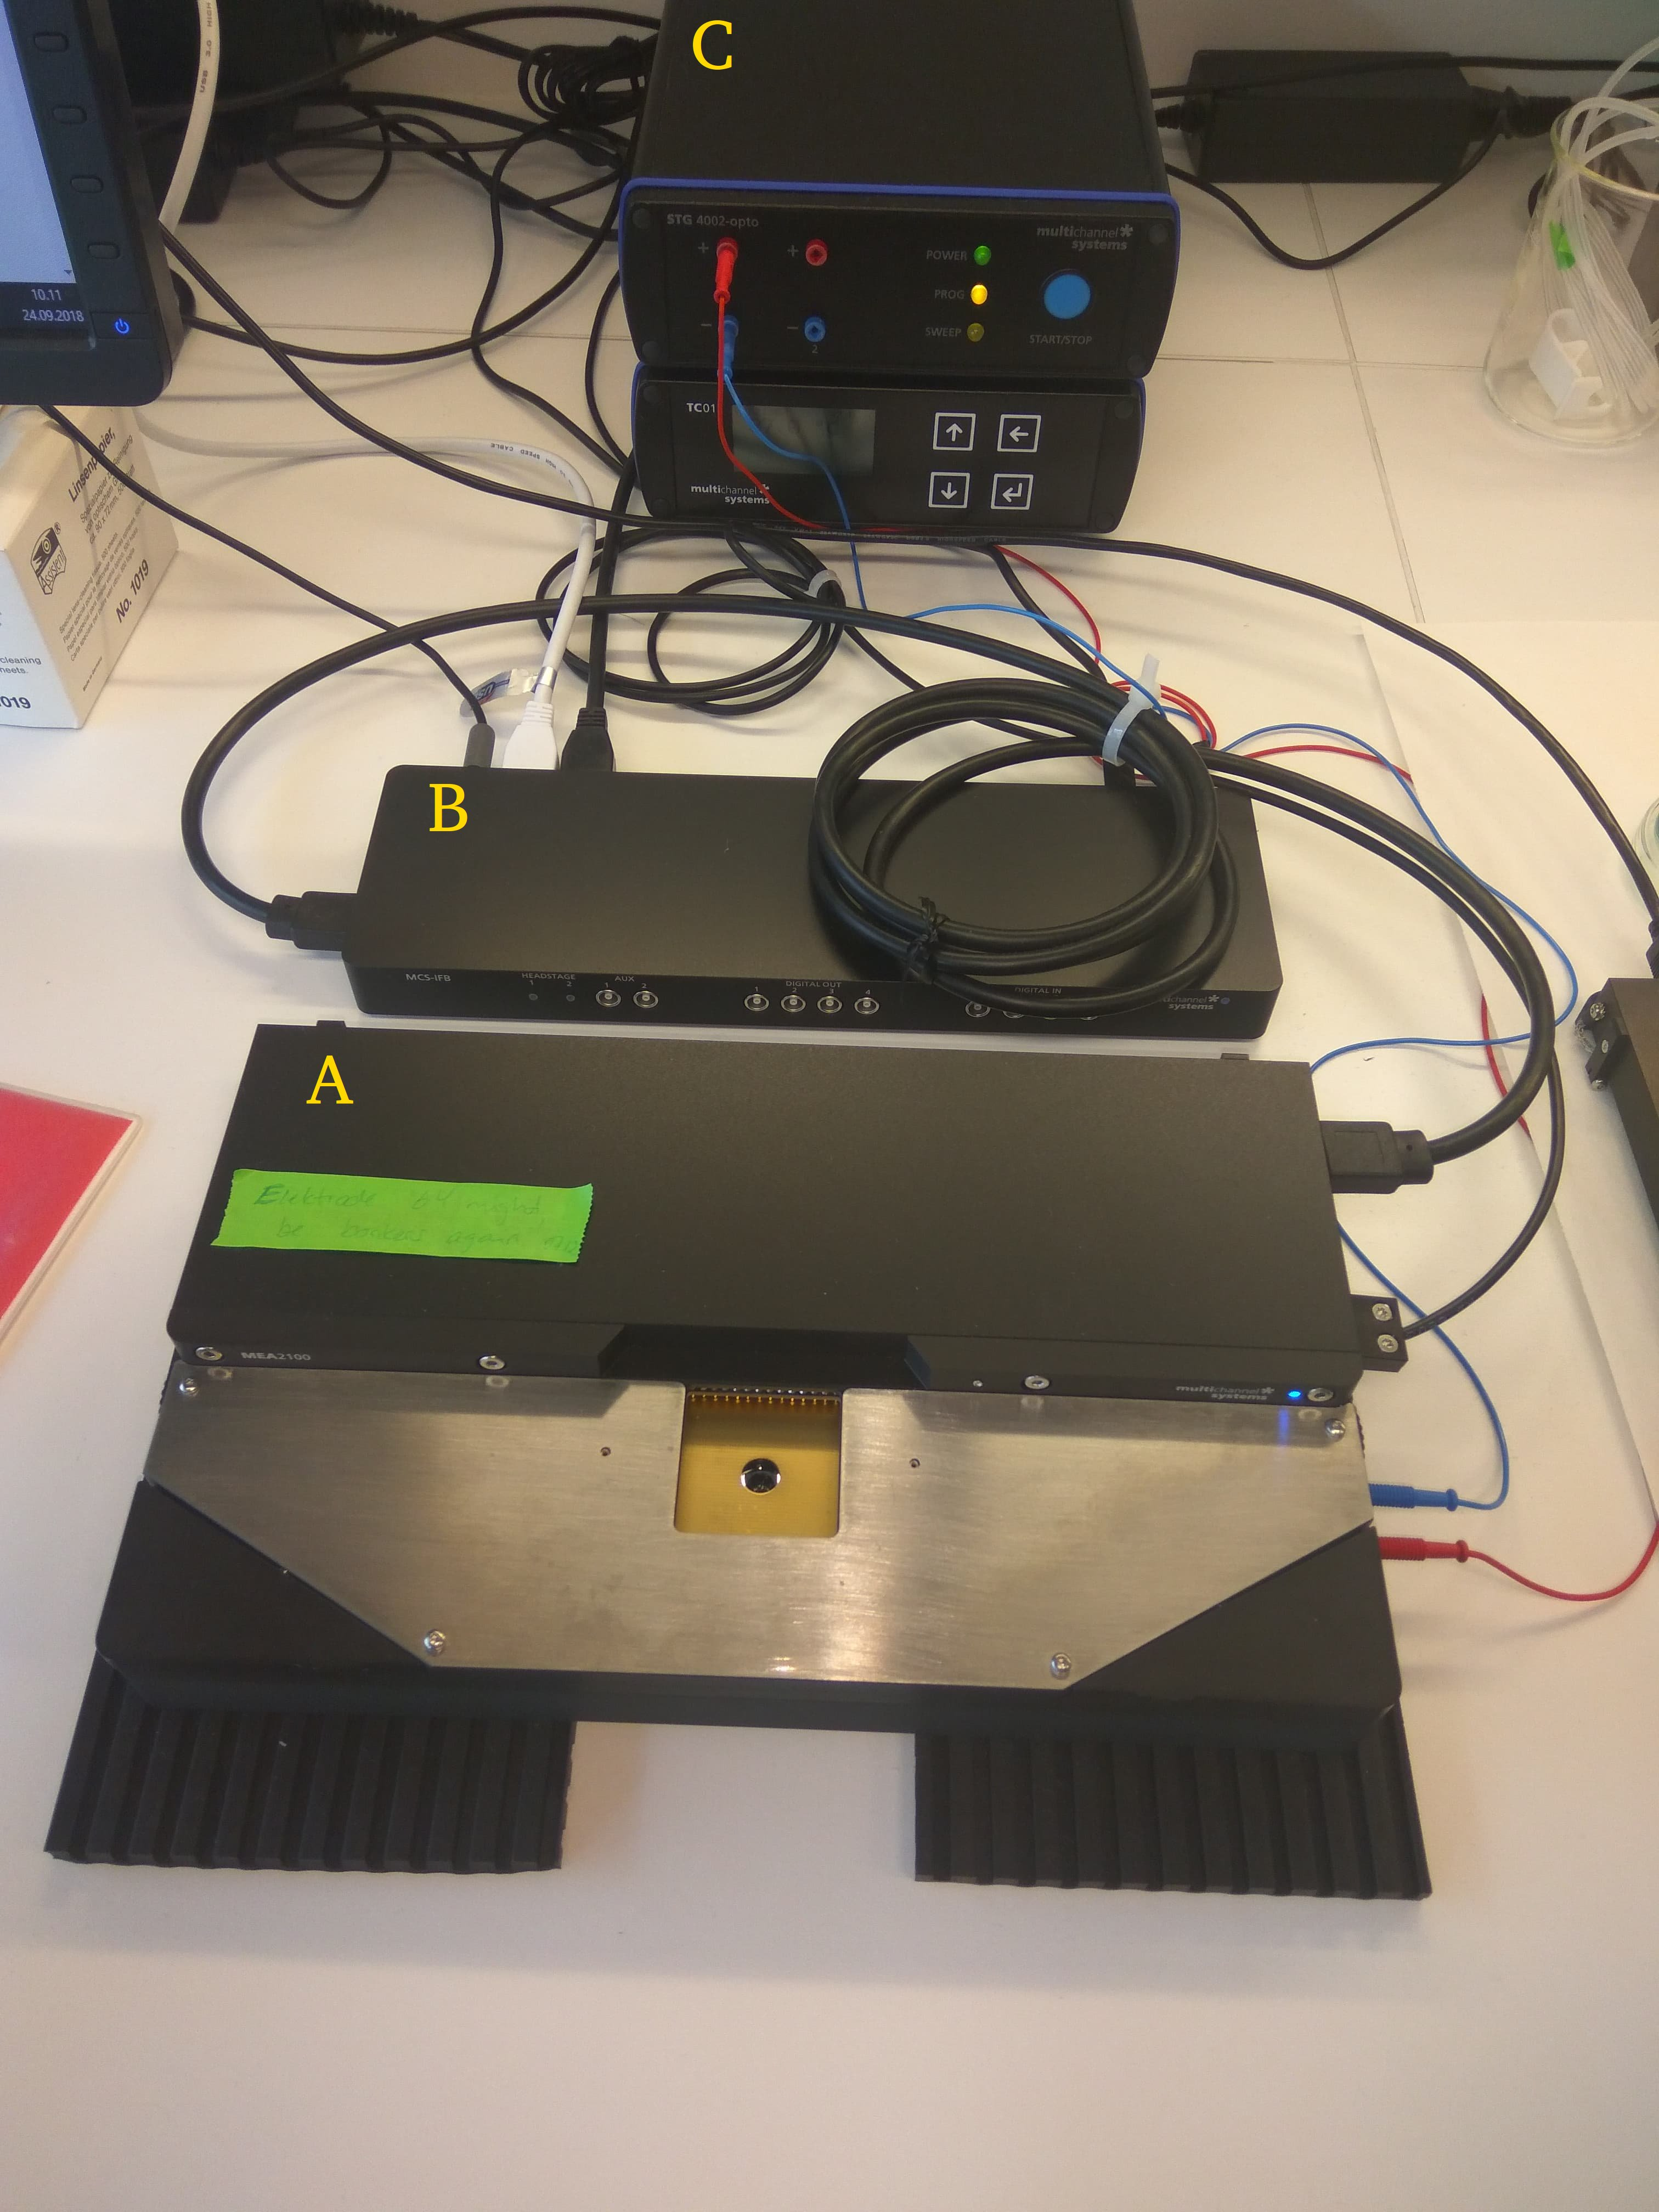
\includegraphics[width=1\textwidth]{fig/LabEquip.jpg}
  \caption[Lab equipment for neural interfacing]{
    An overview of the lab equipment used for interfacing with neurons.
    The components shown are the headstage(A), the interface board(B) and the
    life support(C).
  }
  \label{labEquip}
\end{figure}
\subsubsection{Micro Electrode Array}
Shown in figure \ref{MEAhs}, an MEA
containing a neural culture is slotted into the headstage for measurements.
The MEA can easily be removed, the one shown in the picture is only one
of many MEA's which are kept in an incubator when not experimented on.
These MEA's feature 60 electrodes, which when accounting for the reference
electrode provides 59 individual measurement and stimuli points, evenly spaced
out in a grid.
Each MEA is seeded with a neural culture, i.e once seeded an MEA will
be the host of a single culture, each capable of living for over a year, like
the culture shown in figure \ref{frank}.
\begin{figure}[h!]
  \centering
  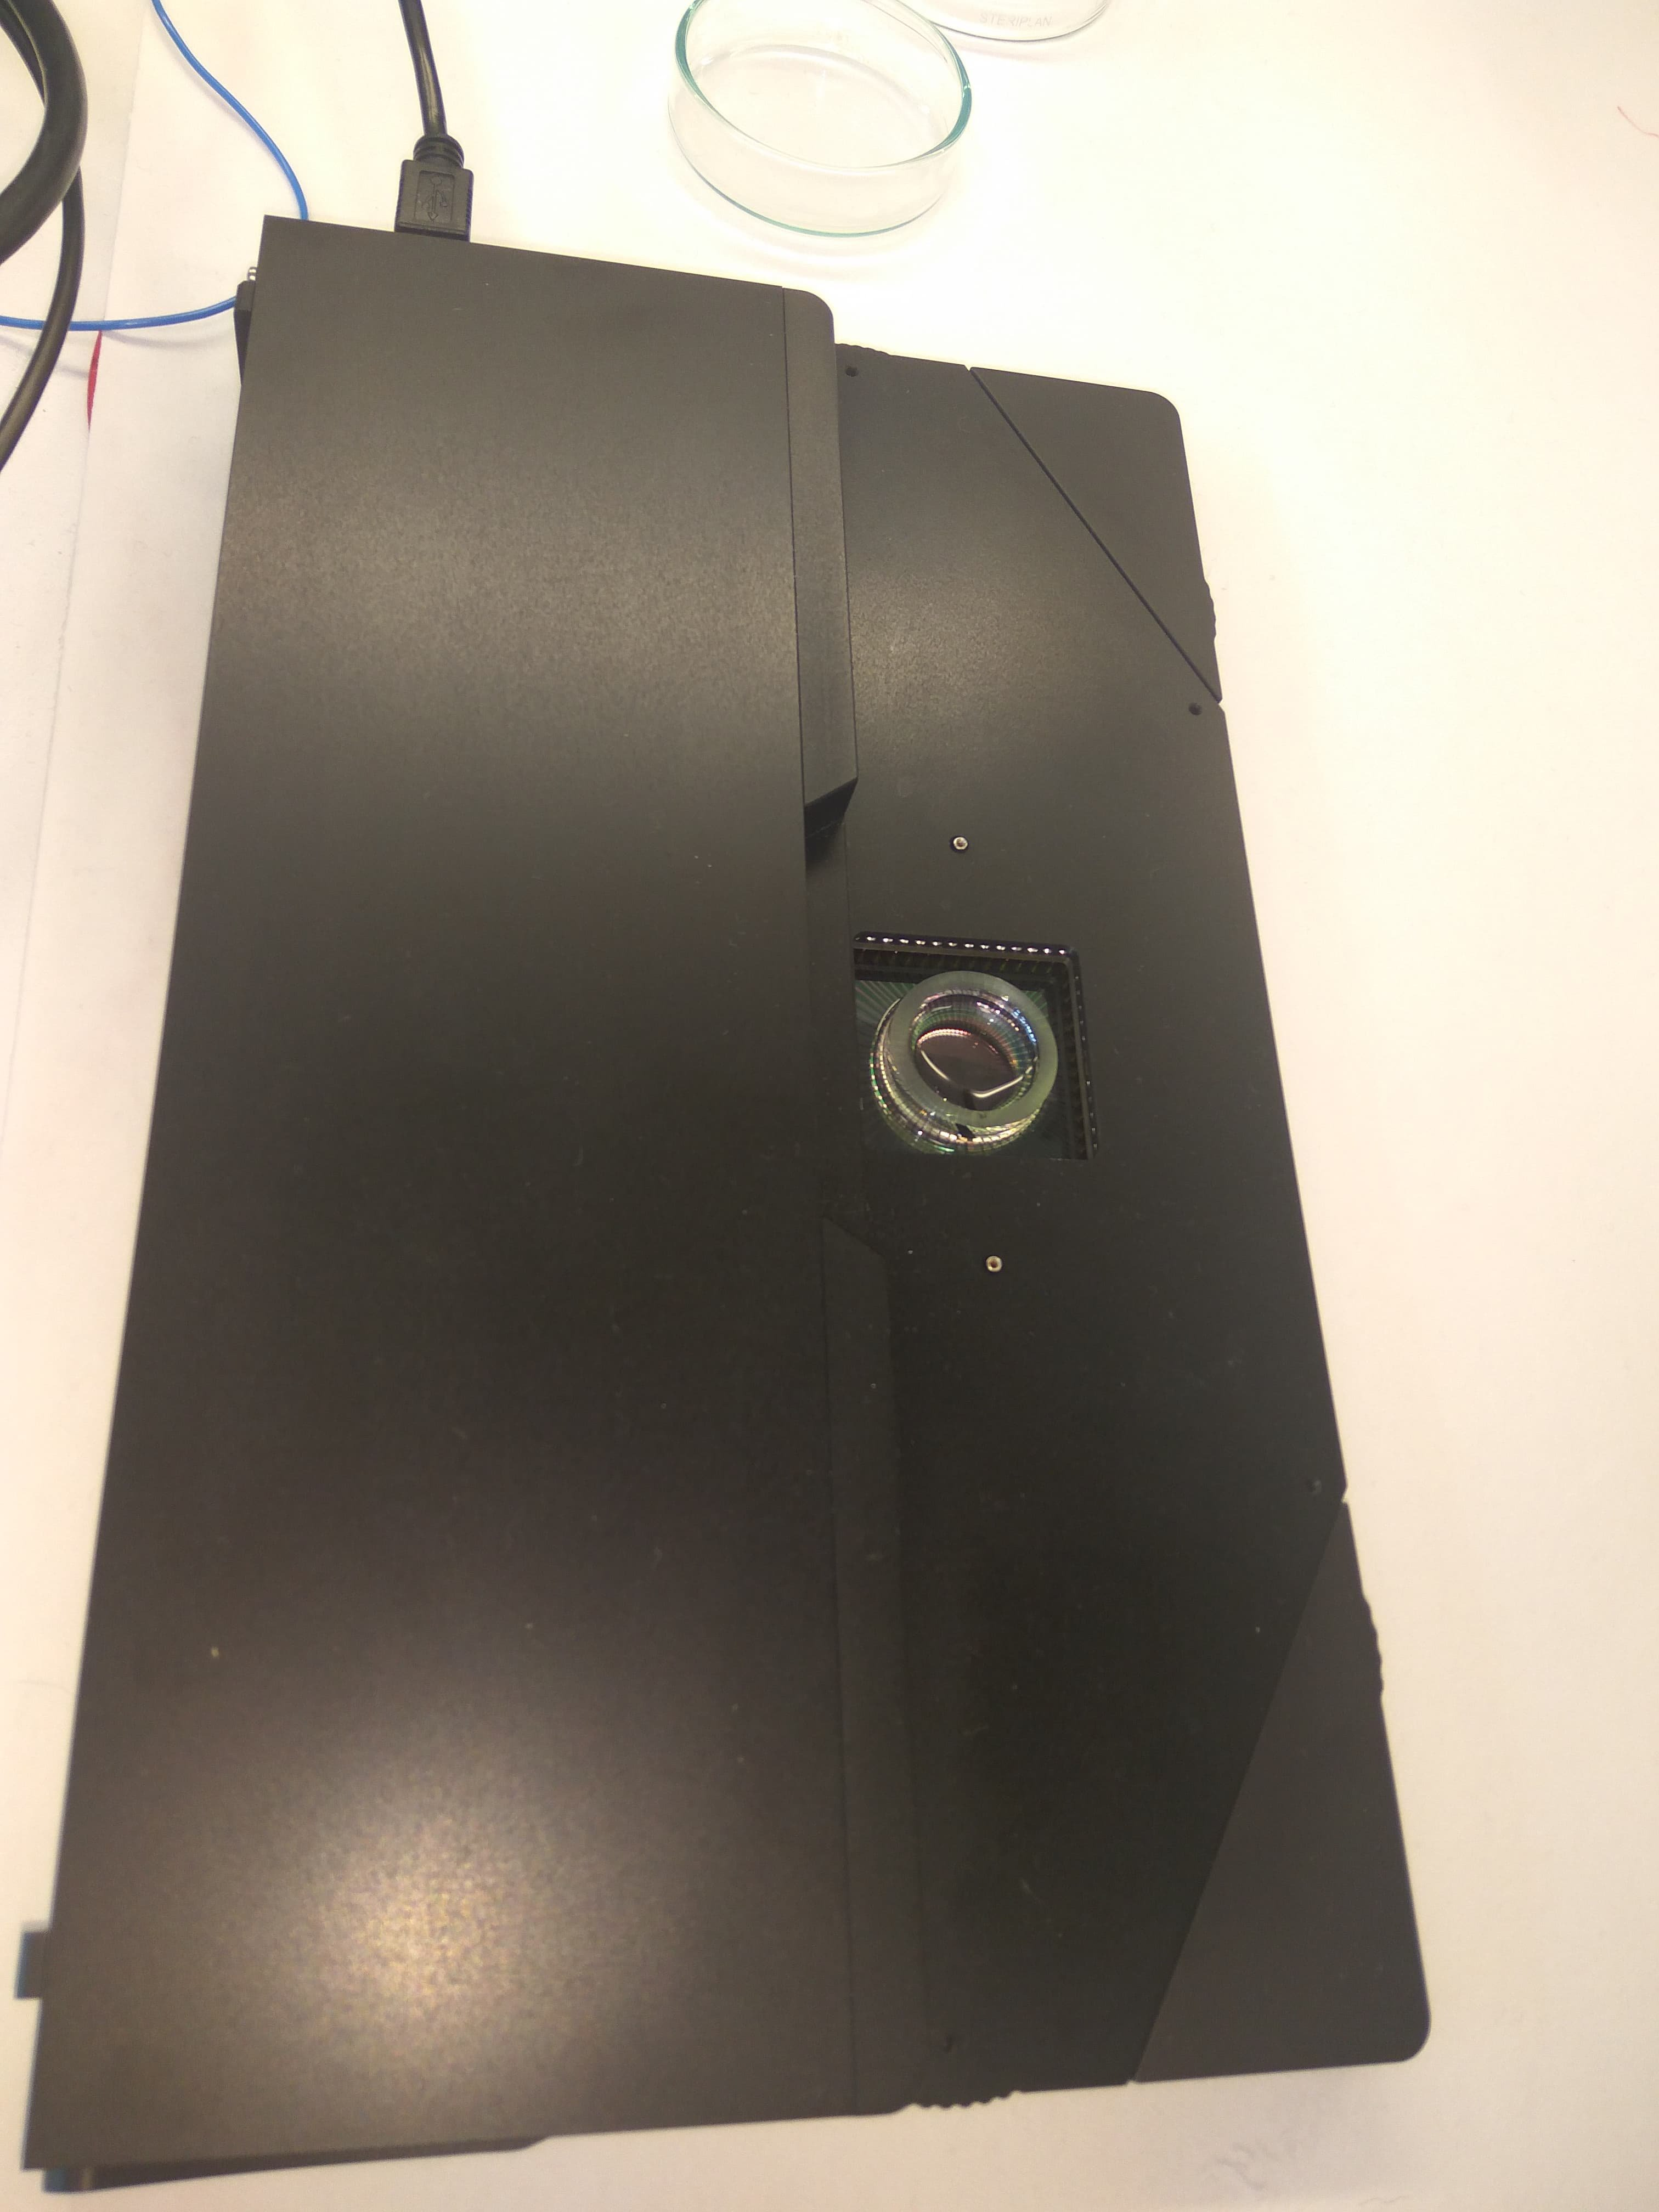
\includegraphics[width=0.7\textwidth]{fig/HS_with_MEA.jpg}
  \caption[MEA2100 headstage with MEA]{
    The headstage with an MEA inserted.
  }
  \label{MEAhs}
\end{figure}
\begin{figure}[h!]
  \centering
  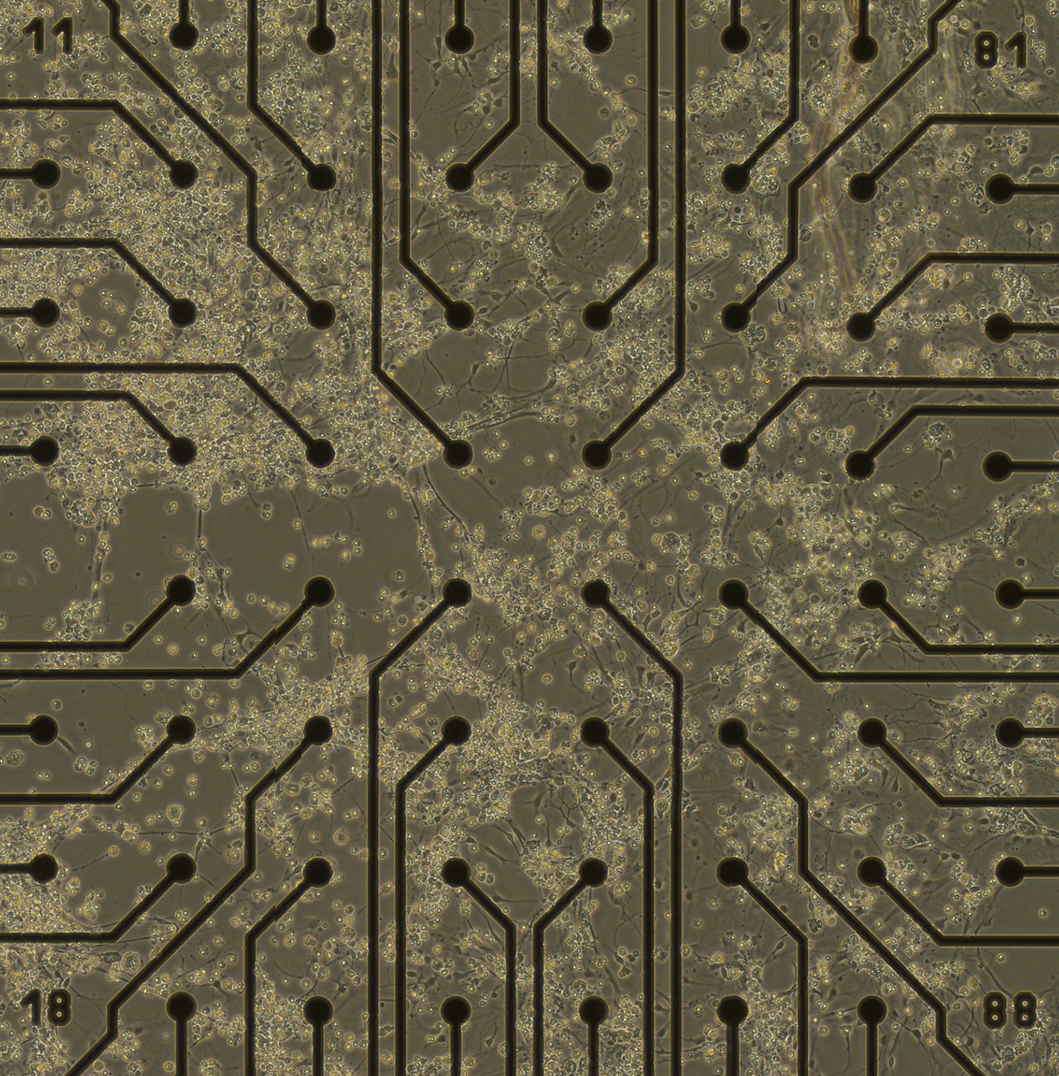
\includegraphics[width=1\textwidth]{fig/frank.png}
  \caption[Microscopic picture of MEA]{
    A neural culture on an MEA seen through a microscope.
    The figure shows a picture taken through a microscope of a culture grown as
    part of the cyborg project.
    The straight black lines are electrodes that can be used to record and apply
    stimuli.
  }
  \label{frank}
\end{figure}
\clearpage
\subsubsection{Headstage}
Equipped with 60 high precision electrodes, shown in figure \ref{openHeadstage}, the
headstage can connect to an MEA when inserted into the measurement bay of the
headstage.
Thanks to the headstage each MEA is relatively expendable as they need only
provide electrodes, leaving the measuerement to the headstage.
\begin{figure}[h!]
  \centering
  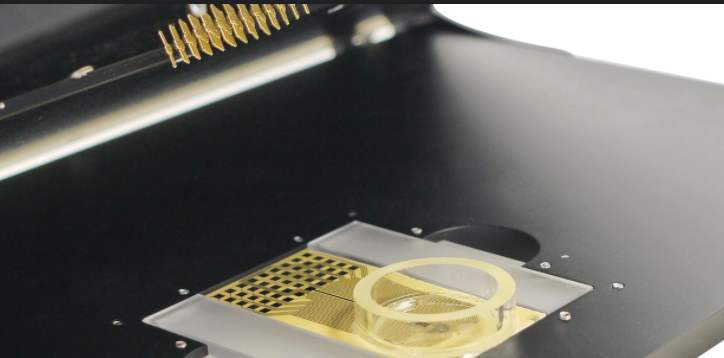
\includegraphics[width=1\textwidth]{fig/hs_placeholder.png}
  \caption[MEA2100 headstage]{
    The MEA2100 headstage. In the very top of the image the rows of electrodes
    that measure electrical activity can be seen.
  }
  \label{openHeadstage}
\end{figure}
\subsubsection{Interface board}
The interface board connects to up to two head-stages and is responsible for
interfacing with the data acquisition computer, as well as auxiliary equipment
such as temperature controls.
For this project, the most interesting feature of the IFB is a user programmable
digital signal processor (DSP), which can access the raw stream of data from the
headstage and issue stimuli.
This DSP has access to the interfacing hardware in the IFB which is otherwise
off limits and not reprogrammable for the user.
% Texas Instruments TMS320C6454 digital signal processor
\section{Software}
Creating a cyborg is a massive undertaking, thus a quite extensive software
suite has been created to make research feasible.
As the system architecture overview in figure \ref{figOverview} hints, the software is the
main body of work performed for this thesis.
Another important detail is the strong emphasis on the dataflow, which is what
connects the individual components.
What goes on inside a component is less relevant compared to the transformation
of data, which is visible from the outside.
Finally, the figure shows a division between two systems, MEAME and SHODAN.
MEAME runs close to the neural cultures, residing on the DSP and lab computer,
and is specialized to interface with the MEA2100 system specifically.
SHODAN on the other hand resides on the other side of the ``network chasm'', and
is closer to a framework, capable of handling any reservoir as long as the
necessary transformations are implemented.
\subsection{MEAME}
An overview of MEAME is shown in figure \ref{figMEAME}, revealing that MEAME internally
consists of two distinct sub-projects exposed by a unified REST interface which
is a common protocol for communicating over network.
While typically REST interfaces imply that a service is public, the MEAME REST
interface is only intended to be used by SHODAN.
%
Behind the REST interface there are two modules: data acquisition and DSP interface.
%
The data acquisition module is responsible for configuring recording parameters
such as sample rate, and starting or stopping recordings, while the DSP interface
provides a very thin layer of abstraction for writing to the DSP memory.
%
Both these modules are built on top of a very thin API provided by the equipment
vendor, making it clear that the closed loop cyborg system is pushing the
equipment further than the vendor intended, for better or worse.
%
In addition to the REST interface, MEAME exposes raw TCP sockets, outputting the
raw waveform data once the lab equipment has been configured.
%
The format of the raw output is shown in figure \ref{figLayout}, which must be
demultiplexed by the receiver in order to separate data into individual
electrode readouts, referred to as \emph{channels}.
%
\begin{figure}[h!]
  \centering
  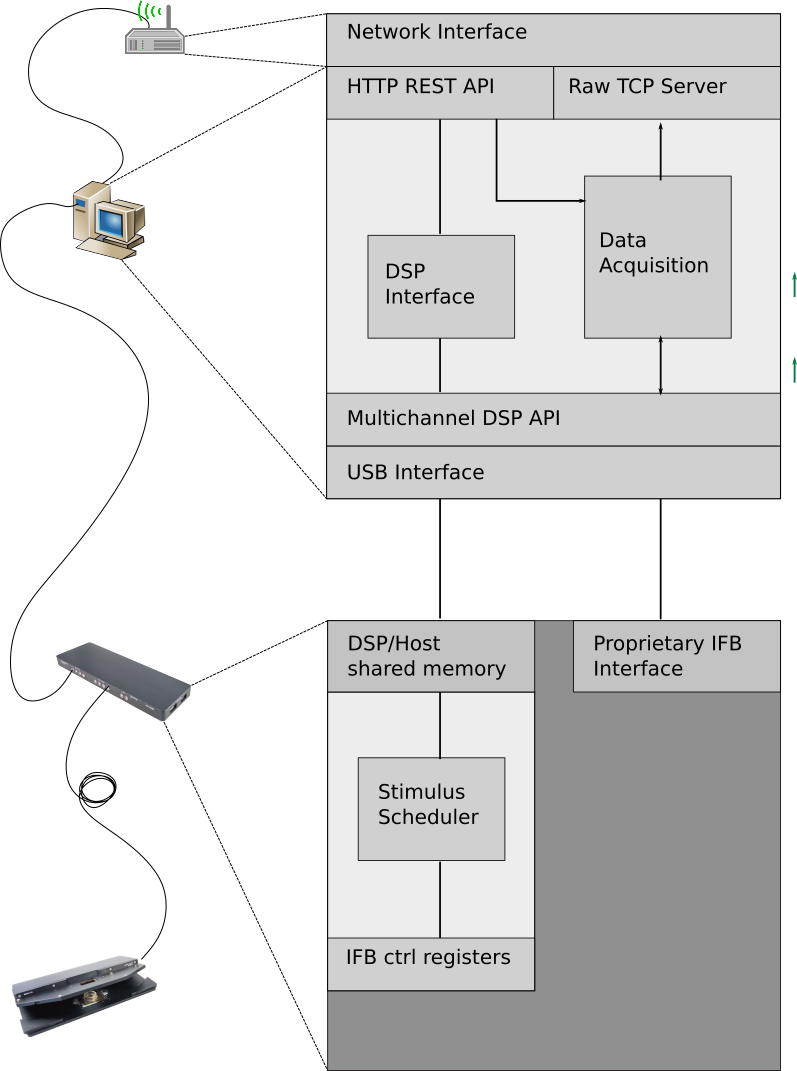
\includegraphics[width=0.5\textwidth]{fig/MEAME.png}
  \caption[Block diagram of MEAME]{
    A block diagram of MEAME.
    The purpose of MEAME is to perform readouts on the neural tissue and
    broadcast this on the network, as well as providing an interface for
    applying stimuli to the neural tissue.
    In the conceptual cyborg shown in figure \ref{figOverviewSimple} the
    functionality provided by MEAME is contained entirely in the box labeled
    ``interface''.
    %% MEAME consists of two subprojects
    %% MEAME is made up of two components residing on the DSP and the connected lab
    %% machine.
  }
  \label{figMEAME}
\end{figure}
\begin{figure}[h!]
  \centering
  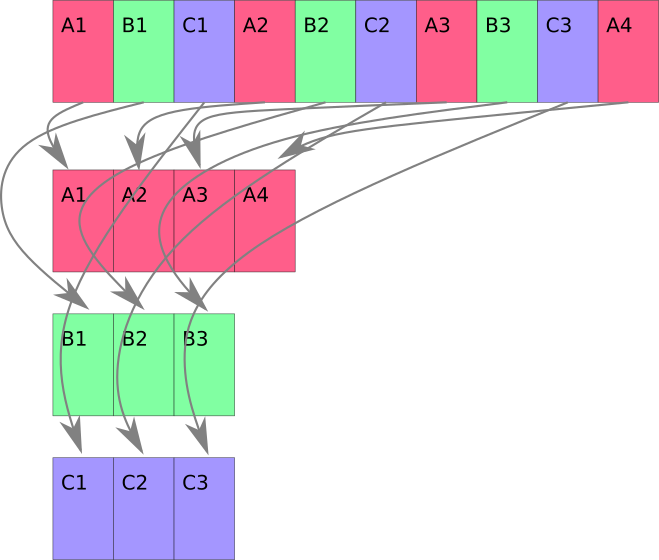
\includegraphics[width=0.5\textwidth]{fig/reorder.png}
  \caption[Data format of neural recordings]{
    The format used when sending recorded neural activity over network.
    The interleaved datastream can be broken down into its individual channels.
    Here a datastream with only 3 streams are shown, whereas the stream is
    normally comprised of data from 60 channels.
  }
  \label{figLayout}
\end{figure}
\subsubsection{MEAME-DSP}
Housed on the IFB, the DSP is not in use during normal operation and thus fully
user programmable.
Communication between MEAME's DSP interface and the DSP itself is done with a
primitive remote procedure call system, implemented using shared memory on the
DSP.
When SHODAN wishes to execute a DSP procedure this is done by submitting a list
of memory writes via the REST interface, and then reading a special register
that is incremented when the procedure call has been executed by the DSP.
This indicates that a new call can be executed, and that return data is valid and
can be safely read.
This rather thin API is admissable because of the fact that MEAME is only
accessed by SHODAN which internally translates procedure calls to memory writes
and reads.
The stim control module maintains a list of \emph{stim groups}, which contain a
list of electrode numbers and a desired frequency.
Consequentially, stimulating neurons is done by specifying which electrodes
should be stimulated, and at which frequency, rather than explicitly sending a
signal whenever stimuli should be applied.
The stimulus group configuration also specifies a pattern for each group, sine
and square respectively.
These patterns can be uploaded by directly writing to memory from SHODAN.
However, for this project simple square waves are adequate.
\subsection{SHODAN}
As shown in figure \ref{figOverview}, SHODAN is responsible for storage, filtering,
generating perturbations and maintaining the core RC loop.
During an experiment SHODAN can be divided into two parts, reservoir interfacing
shown in figure \ref{figSHODANiface}, and and the core RC loop which can be seen
in the overview figure \ref{figOverview}.
The former can in turn be subdivided into input and output processing with
regards to the main RC loop.
\begin{figure}[h!]
  \centering
  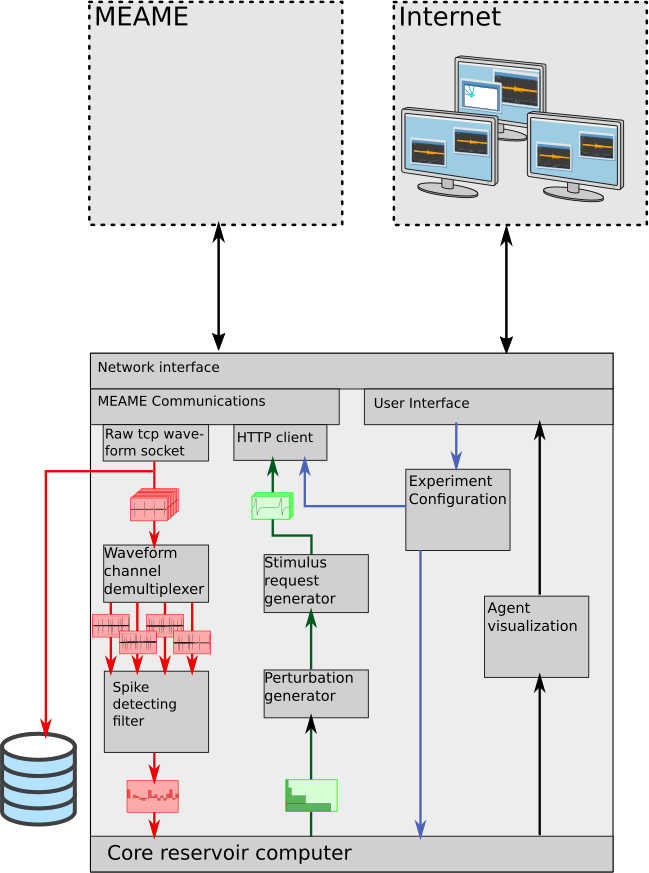
\includegraphics[width=0.5\textwidth]{fig/SHODANfrontend.png}
  \caption[Block diagram of SHODANs frontend]{
    A block diagram of the frontend of SHODAN.
    The frontend of SHODAN, responsible for demuxing the datastream (shown in
    figure \ref{figLayout}) and
    preprocessing the input data (shown in figure \ref{figWaves}) before handing it
    over to the core reservoir computer.
    The frontend is also responsible for translating sensory data from the core
    reservoir computer to neuron-compatible perturbations (shown in the right
    part of figure \ref{figGenericSpecific}).
    The frontend is also responsible for hosting a web-interface allowing
    configuration and visualization of data through a browser.
    In the conceptual cyborg shown in figure \ref{figOverviewSimple} the
    functionality provided by SHODANs frontend is contained in the boxes labeled
    ``interface'' and ``feedback processor''.
  }
  \label{figSHODANiface}
\end{figure}
\subsubsection{Input Processing}
The MEAME comms interfacing module mirrors the corresponding interface exposed
by MEAME, consuming raw waveform data over a TCP connection, and configuring
experiment parameters and issuing stimuli requests using a HTTP client.
The transformation of data is shown in figure \ref{figWaves}:
First the channel demultiplexer splits the raw datastream from the TCP sockets into
individual channels before entering the filtering module.
Next, the filtering module is responsible for translating the raw waveforms to a
format that can be utilized by the main RC loop, which in the current
implementation is done by a basic ``spike detection'' transform where a binary
spike event is recorded whenever a certain voltage threshold is reached,
followed by a short cooldown where the detector is disabled for a short period
before it can detect the next spike. 
Finally, the spikes are input into a moving average filter, smoothing out the
staccato spike/no spike filter output to the amount of spikes that have occured
between $t$ and $t - \Delta t$ where $\Delta t$ is in the order of 100ms to 1000ms.
The final input to the core RC loop is a vector of values, one for each channel
that can be periodically sampled.
As the data crosses the boundary to the core RC loop, its shape reveals little
facts about its origin.
For any other reservoir it would be just as natural to translate the output
dynamics to a vector of scalars, thus for any reservoir the filter module is
what translates from specific to generic.
\begin{figure}[h!]
  \centering
  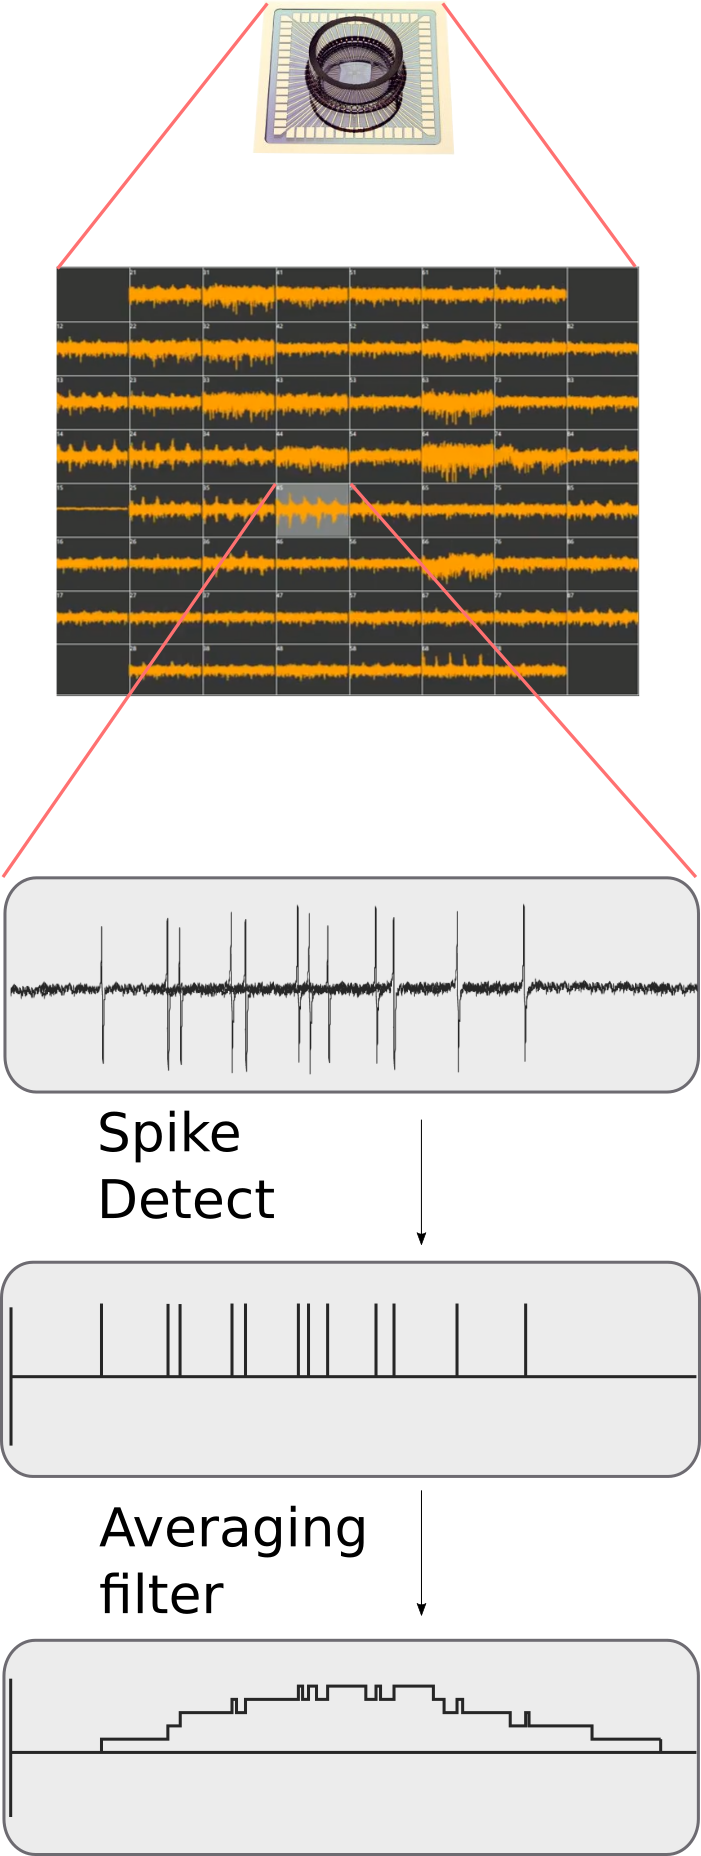
\includegraphics[width=0.5\textwidth]{fig/system4.png}
  \caption[Preprocessing of neural data]{
    The preprocessing pipeline in more detail.
    The figure shows how neural activity is sampled and preprocessed to
    be compatible with the input layer of the reservoir computer.
    For each channel a spike detector singles out spikes which is then input
    into an averaging filter.
    In the conceptual cyborg shown in figure \ref{figOverviewSimple} the
    preprocessing is contained in the box labeled ``interface''.
  }
  \label{figWaves}
\end{figure}
\subsubsection{Output Processing}
Being the dual of the Input processor, the output processor does the same thing
in reverse, transforming data from generic to specific.
In the figure \ref{figSHODANiface} the output of the main RC loop is shown as a
list of distances, but this is merely our interpretation of the data.
The underlying shape is just the same as the output of the filter from the input
processor: a vector of scalars which does not hint that these particular scalars
encode distances.
Since the goal of the project is to create a cyborg, the focus is naturally on
robotics, virtual or not, but the main RC loop can just as well handle other
tasks such as classifying images, and the resulting output would still be
expressed as a vector of scalars.
Figure \ref{figGenericSpecific} shows this duality between the input and output
processor: Just as the input processor masks the identity of the reservoir from
the core RC loop, the output processor masks the identity of the task being
performed!\par
The datapath of the output processor is rather similar to the input processor
with the perturbation transform module serving the same purpose as the filter in
reverse, turning scalars into frequency ranges.
In the figure an additional module is shown, transforming a stim request into a
set of memory writes for the DSP as described in the MEAME section, but this is
just a practical matter added for completeness.
\begin{figure}[h!]
  \centering
  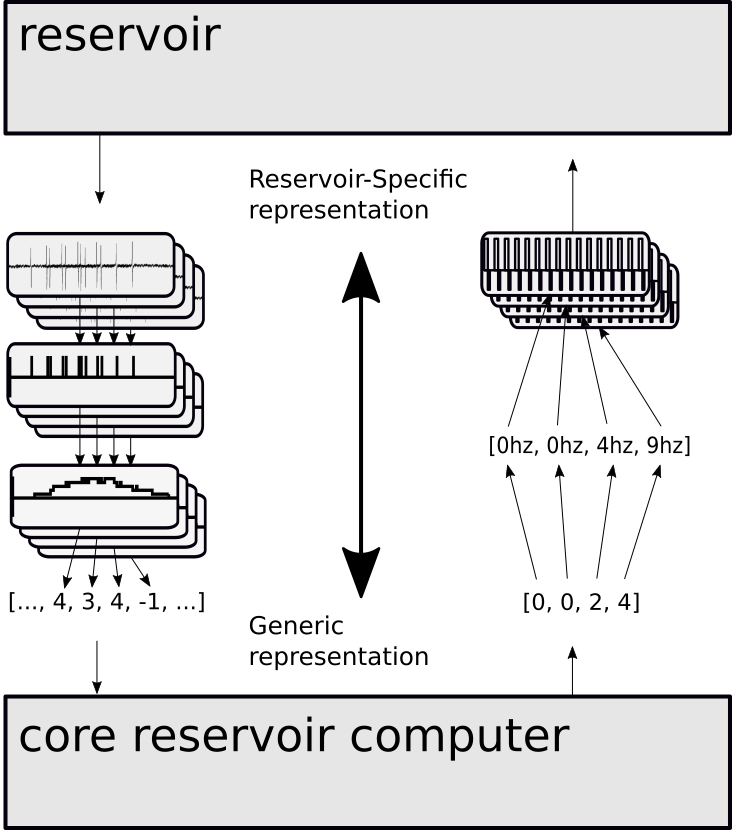
\includegraphics[width=0.5\textwidth]{fig/genericSpecific.png}
  \caption[Anonymization of data between reservoir and reservoir computer]{
    Figure showing the ``anonymization'' that happens between reservoir and core
    reservoir computer.
    When using neural tissue as a reservoir, the preprocessing stages transforms
    the recordings from neural tissue to a vector of scalars which would be
    indistinguishable from any other reservoir.
    Likewise, the perturbations generated from the perturbation generator does
    not reveal anything about what sort of task the neurons are actually
    performing since the sensory input is simply reduced to a square wave!
  }
  \label{figGenericSpecific}
\end{figure}
\subsubsection{Core RC Loop}
In the conceptual cyborg (figure \ref{figOverviewSimple}), all of the software
described previously can be fit into the interface between the ANN and MEA.
The core of the reservoir computing system is the ANN readout and the robot
control module, but the concept leaves out a very important piece of the puzzle:
How can the correct ANN readout layer be chosen?
The Core RC loop consists of three components, the robot control, the RC
filter, and the reservoir performance evaluator.
Just as the robot control does not have to be an actual robot, the RC filter
can employ any filter, it does not necessarily need to be an ANN.
The last module is what separates SHODAN from a classical reservoir computer.
In classical reservoir computing the reservoirs themselves are fairly static,
exhibiting little changes in behaviour over time.
A reservoir computer using a random boolean network can store an RBN in memory
and access this data to reconstruct the experiment at any time.
This simplifies the task of training the RC output layer, since the reservoir
will not change between runs.
Unlike digital RBNs, neural cultures have no reset button, their behaviour
changes both long term and short term.
Long term, a cluster of neurons might ``emigrate'' away from an electrode, new
connections form and old connections wither.
This process happens over days and weeks, but change also happens on a short
basis, both due to natural fluctuation, and because of the fact that no two
experiments are truly independendent, there are no ways to make neurons forget
and revert to previous behaviour.
The solution to this problem is to back link the robot control to the RC filter
via a performance evaluation module, which creates a feedback loop capable of coping
with the moving target presented by a neural culture.\par
\subsection{Storage And User Interface}
This section will feature the UI and a description of the database system and
the sort of offline analysis that can be done.
It's not that interesting, but it does provide a significant boost to the
usability of the system.
%
\section{Current State}
MEAME and SHODAN are both still in development and are far from complete.
All functionality described in this chapter has been implemented and is in a
running state, but the stimuli control module that is responsible for applying
voltage to the electrodes does not work correctly.
This means that the closed loop system does not work at all until the issue can
be fixed.
This frustrating issue reflects how the closed loop system goes far beyond the
intended use for the lab equipment, which is marred by poor software and
nonsensical documentation, leading to development often being frustrating process of
reverse-engineering rather than engineering.
While this flaw means the system does not fulfill its purpose, it's enough to
verify that the remaining modules work.
Recordings can be made and played back, which means that MEAME/SHODAN is already
able to provide a better storage solution than the vendor provided solution.
MEAME and SHODAN are available on github
\cite{MEAME_github}\cite{SHODAN_github}\cite{MEAME_DSP_github}
%%% Local Variables:
%%% mode: latex
%%% TeX-master: "../main"
%%% End:
